\documentclass[UTF8]{ctexart}
\usepackage{mathtools,wallpaper}
\usepackage{lmodern}
\usepackage{float}
\usepackage{t1enc}
\usepackage{pagecolor}
\usepackage{booktabs}
\usepackage{amsmath}
\usepackage{amsthm}
\usepackage{graphicx}
\renewcommand{\(}{\left(}
\renewcommand{\)}{\right)}
\begin{document}
\title{算法设计 HW06}  
\author{Xun Ying}
\maketitle

\paragraph{Q1} 

To prove it is NP-complete, we first prove it is in NP. As a clique S can be a certificate, and we
can verfiy whether S is a cllique and whether $\vert S \vert = \frac{n}{2}$ in polynomial time. So, it is in NP.

Then, we want to prove it is NP-complete. We can make a reduction from Clique. 
We have a clique $G_{1} = (V, E), k$, so we can make a similar $G' = (V', E')$ in $G$.

If $k \leq \frac{\vert V \vert}{2}$, we can add $\vert V \vert - 2k$ vertices to $V'$, and add edges between them and all vertices in $V'$.
So, the G' has a $\vert V' \vert$ of size $2\vert V \vert - 2k$. So, if there is a clique of size k in G,
so there is at least a clique of size $\vert V \vert - k \geq \frac{\vert V' \vert}{2}$ in $G'$. And if there is a 
clique of size $\frac{\vert V' \vert}{2}$ in $G'$, so there is also a clique of size $\vert V \vert - k -(\vert V \vert -2k) = k$ in $G$.

If $k > \frac{\vert V \vert}{2}$, we can add $2k - \vert V \vert$ vertices to $V'$, and all of them hava no edges connected to them.
So, the G' has a $\vert V' \vert$ of size $2k$. So, if there is a clique of size k in G, then there is a clique of size $k > \frac{\vert V \vert}{2}$ in $G'$.
And if there is a clique of size $k > \frac{\vert V \vert}{2}$ in $G'$, then there is a clique of size $k$ in $G$.

Therefore the problem is NP-complete.

\paragraph{Q2}

(a) First when $k = 1$, it is trival.

Then, when $k \geq 2$. We first prove it is in NP. We can use a spanning tree T with maximum degree k, and
it is easy to prove that we can use polynomial time to verify whether T is a spanning tree and whether the maximum degree of T is k.

So, we just want to prove it is NP-complete. We can make a reduction from Hamiltonian Path. Given a Hamitonian Path $P \subset G= (V, E)$.
We can make a spanning tree $T \subset G' = (V', E')$ with maximum degree at most k by following steps: We add $(k-2)\vert V \vert$ new vertices
from G to $G'$ and connect each node in G with $k-2$ different new vertices. So, if there is a Hamiltonian Path P in G, then there is a spanning tree with maximum degree k=2 in $G'$.

If the vertices in $G$ connect to k-2 new vertices have degree at most k in $G'$, the vertices in G have degree at most 2 in $G$. So, if there is a spanning tree with maximum degree k in $G'$, then there is a spanning tree with maximum degree at most 2 in G.  
SO, there is a Hamiltonian Path in G.

So, the problem is NP-complete.

(b)Similarly, it is easy to prove it is in NP. 

So, just like (a), we can make a reduction from Hamiltonian Path. Given a Hamiltonian Path $P \subset G= (V, E)$. We can make a spanning tree $T \subset G' = (V', E')$ with maximum degree at most k in $G'$by the same way in (a) when k is fixed.

So, if there is a Hamiltonian Path in G, then there is a spanning tree with maximum degree at most 2 in G. 
So, we can add k-2 edges from each vertices in G to the new vertices in $G'$, and the maximum degree of the vertices in G is at most k. So, if there is a spanning tree with maximum degree at most k in $G'$.

What's more, if the vertices in G connected to k-2 new vertices have degree at most k in $G'$, then the vertices in G have degree at most 2 in G. So, there is a 
spanning tree with maximum degree at most k in $G'$. So, there is a spanning tree with maximumdegree at most 2 in G, so there is a Hamiltonian path inn G.

So the problem is NP-complete.


\paragraph{Q3}
Amazing idea!!!!!

First, prove it is in NP, as a color c of each vertice can served as a certificate, and we can verify whether the color is legal in polynomial time.

Then, we can make a reduction from 3-SAT. Given a 3-SAT formula $\phi = C_{1} \wedge C_{2} \wedge \cdots \wedge C_{m}$, and the variables are $x_{1}, x_{2}, \cdots, x_{n}$. So, we can construct a graph
G=(V, E) in the problem as follws:

We can first create a triangle in G with 3 verticles {T, F, A} and T stands for true and F stands for false.
What's more, it is a triangle, so we can use three colors to color. Then, for each varibles, we can add a triangle with 3 verticles ${x_{i}, \neg x_{i}, A}$ and $x_{i}$ stands for the i-th variable. And we can use 3 colors to color them. 
So, the graph is like below:
\begin{figure}[H]
    \centering
    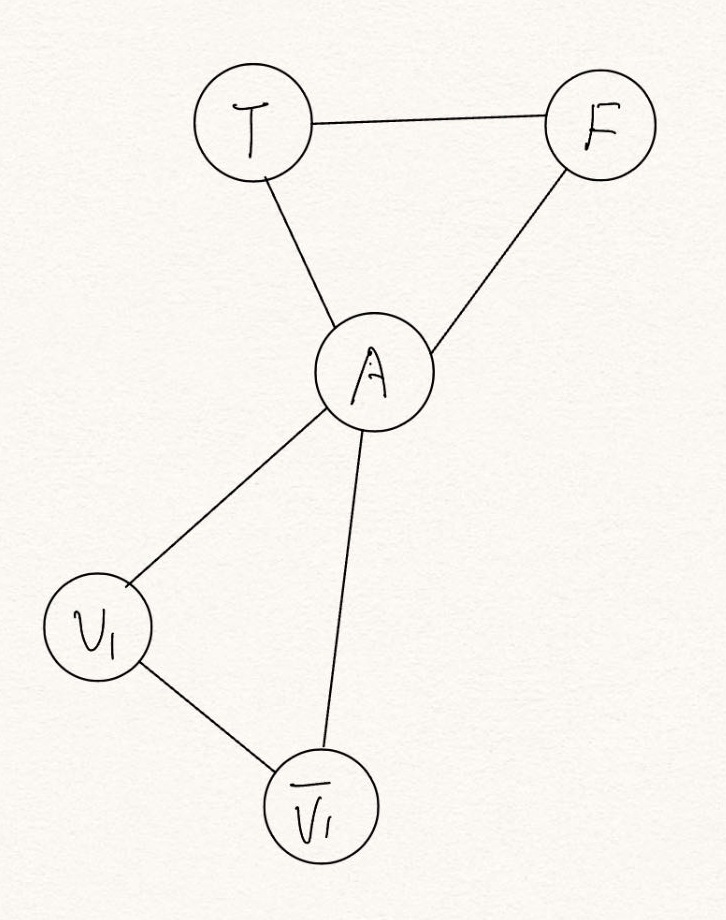
\includegraphics[width=7cm,height=8cm]{1.jpg}
    \caption{sample}
    \end{figure} 

If G is 3-color, then either $v_{i}$ or $\neg v_{i}$ gets true as they are connected to A.
and the other gets F. So, we can use the color to replace the value of $v_{i}$. Also, if the formula is satisfiable, then we can use the value of $v_{i}$ to color the graph.
And the color is 3-color.

So, we next need to draw the clauses. For each clause $\phi_{i} = a \vee b \vee c$, we can draw a graph by OR-gadget as below:
\begin{figure}[H]
    \centering
    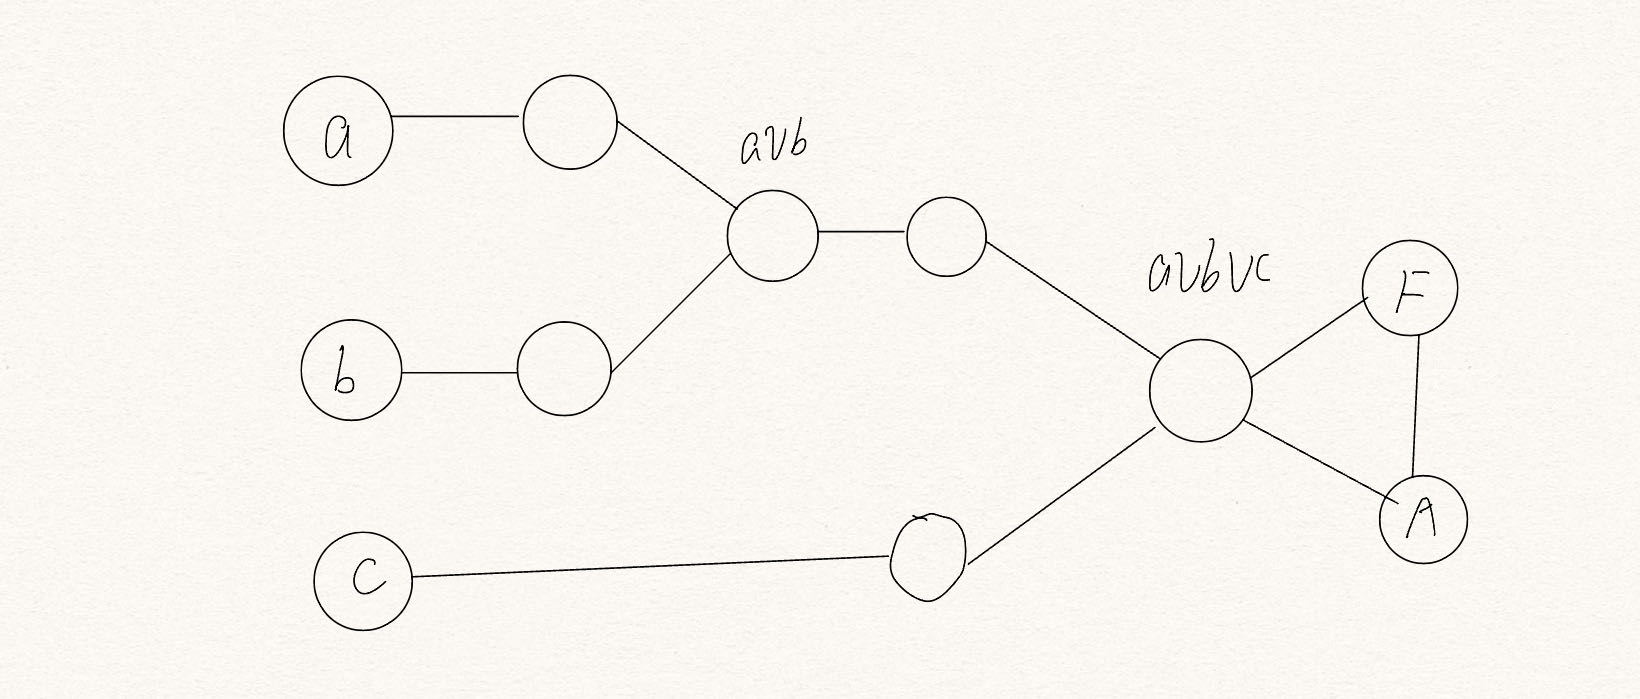
\includegraphics[width=12cm,height=7cm]{2.jpg}
    \caption{sample}
    \end{figure} 

If a and b are all F in 3-color, then $a \vee  b$ must be F, so it is an or gate. So, if a,b,c are all F, the graph cannot be colored by 3-color, 
which means the formula cannot be satisfied. 

If a or b or c has at least one T, WLOG, we assume a is T, then the $a \vee b$ is T, so $a \vee b \vee c$
is T, and the graph is 3-color. So, the formula is satisfied.

As a result, for each $C_{i}$, we can draw a graph, we can connect the last $a \vee \cdots e$ to the O and F node in the triangle.
So, if there is a 3-coloring in the graph, then the formula is satisfied and the value is the color.

On the other hand, if $\phi$ is satisfied, then, we can color  ${x_{i}, \neg x_{i}}$ according to the assignment of $x_{i}$, and the color is unique.
Then, we can color the OR-gadget according to the assignment of the variables, and the color is unique. So, the graph is 3-color.

Therefore, the problem is NP-complete.

\paragraph{Q4}

collaborate :蒋松霖

difficulty: 1 and 2 is normal, 3 is very, very, very hard.




\end{document}